\chapter{MACHINE-READABLE CHANGE LOG}\label{ch:changelog}

\section{Introduction}

\Glspl{log} explain the differences between \glspl{version}; however, they are often only available in human-readable formats.
Readability puts a limit on the length and extent of the \gls{log} since a human will need to write it.
Manageable change descriptions become difficult with large data sets featuring many changes, or data sets that change often, but large data sets are exactly the data sets which need \glspl{log} the most.
Automating the process will allow more data sets to provide change documentation in a timely fashion for data sets.
Encoding the change logs with structured data will provide a means for users to efficiently consume change information.
The additional encoding will inflate the size of a standard change log which becomes an issue with the \glspl{log}.


\Glspl{log} were generated for two data sets, the ``Global Database on \textsuperscript{3}He/\-\textsuperscript{4}He in on-shore free-circulated subsurface fluids" data set and the Paragenetic Mode for Copper Minerals database.
Following the practices of other \glspl{log}, the documents present before and after values for comparison which can be seen in Figure \ref{changelog_zoomed}.
\begin{figure}
	\centering
	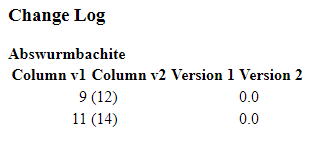
\includegraphics[scale=0.80]{figures/Changelog-zoomed.png}
	\caption{Abswurmbachite entry in the Copper Dataset Change Log}
	\label{changelog_zoomed}
\end{figure}
The change logs identify challenges to adopting thorough change logs as a practice in versioning data sets.

\subsection{On the Importance of Change Log Automation}

The \gls{nasa}'s \gls{clpx} collects ice measurements from a wide number of sites in the arctic \cite{CLPX}.
The data was published originally in ASCII, but the data was later ported into shapefiles as well.
A known issue with the transition was that comments in the Summary data set were left out due to format limitations.
A \gls{log} was created to determine whether additional differences existed within the two formats.

The initial problem with forming a \gls{log} is that rows in the data did not include unique identifiers to align \glspl{attribute} within the \glspl{version}.
A unique tuple, using values from five columns of the data, was created to match rows together since the order of the rows did not correspond between the two formats.
An immediate problem that resulted was some differences occurred within the columns necessary to form the unique tuple, namely some values disagreed by 0.5.
Following the correction, the data could be correctly aligned.

The \gls{log} found that for columns ``soil sample A" (SL\_A) and ``soil sample B" (SL\_B), many entries consistently disagreed between \glspl{version}.
Disagreements resulted from values being recorded with `y' or `n' for a number of values but with numbers for the rest.
Since the values in the shapefiles are stored in a database format, a column must conform to a pre-specified type, causing the character encodings to appear as 0s in the shapefiles.
Additionally, the columns experienced 0.5 misalignments and null values of -999.0 being encoded as 0.
The columns are encoded as integers, causing the disagreement.

With further investigation, misalignment in the values caused repeated inquiries into differences between expected and reported values.
Parsons et al. \cite{CLPX2} state that the, ``text files are the primary archival format of the data."
The solution resolve differences between the formats was to defer to an official version rather than compute or provide change information.
The deference to a different format, unfortunately partially undermines the benefits of increased accessibility provided by the shapefile format.

\section{Encoding a Change Log}

Very little natural language is used in the \gls{log} to regularize the format and improve compatibility with \gls{rdfa}.
The \glspl{log} follow a common format with three sections as seen in: Additions, Invalidations, and then Modifications.
The sections may be further grouped by column or row additions.
The division means that \glspl{change} are not published into the \gls{log} as they are found, but instead organized and grouped beforehand.

Employing \gls{rdfa} means that the document must be written using \gls{html} formatting.
Listing \ref{rdfa_list} shows the text necessary to layout the first four lines of Figure \ref{changelog_zoomed}, showing \glspl{modify} for the Abswurmbachite mineral from the Copper Minerals database.
While the content only shows four lines, the underlying markup takes up three and a half times as many lines.
Line 2 of Listing \ref{rdfa_list} states that all following resources will be \glspl{attribute} of Version 1.
\begin{listing}
	\begin{minted}[linenos, frame=lines, framesep=2mm, breaklines]{HTML}
<h3>Change Log</h3>
  <div about="Version1" rel="vo:hasAttribute">
    <div resource="v2:Abswurmbachite" typeof="vo:Attribute">
    <span style="font-weight:bold" property="http://www.w3.org/2000/01/rdf-schema#label">Abswurmbachite</span>
    <table rel="vo:Undergoes">
      <tr  about="ChangeAbswurmbachite12" typeof="vo:Change">
        <td align="right" rev="vo:Undergoes" resource="v1:AttributeAbswurmbachite12v1" typeof="vo:Attribute"> 9</td>
        <td property="vo:resultsIn" resource="v2:AttributeAbswurmbachite12v2" typeof="vo:Attribute">(12)</td>
        <td>          </td>
        <td>       0.0</td>
        <span about="Version1" property="vo:hasAttribute" resource="v1:AttributeAbswurmbachite12v1"></span>
        <span about="Version2" property="vo:hasAttribute" resource="v2:AttributeAbswurmbachite12v2"></span>
      </tr>
</table></div></div><br>
	\end{minted}
	\caption{Abswurmbachite RDFa\label{rdfa_list}}
\end{listing}
Line 3 defines such an \gls{attribute}.
Lines 5 through 8 define the \glspl{change} Abswurmbachite undergoes.
Because \gls{rdfa} allows the statements to be embedded within the content, the triples can appear along with the text they describe.
Lines 11 and 12 define complete triples which do not appear in the visible document.
The lines complete the graph, but must be included in \gls{html} span tags because \gls{rdfa} only allows a single triple within each tag.
Modifying the tags' order so that the spans are unnecessary would cause the visible content to appear in a confusing and disorganized order, rendering the document machine-readable but not human-readable.


After encountering the limitations of using \gls{rdfa} to include the versioning graph into the change log, \gls{jsonld} was used.
The \gls{json} data does not need to conform to the structure or ordering of visible content in the change log.
Listing \ref{json_list} provides the alternative encoding of the Abswurmbachite entry from \gls{rdfa}.
The entry is significantly longer, almost three times longer than the \gls{rdfa} entry and ten times longer than the original visible content.
Instead of including all the data in the beginning or end of the document, each change block is separated into the particular \textit{div} section for that change.
This choice allows consumers to extract pertinent change information without needing to ingest the entire \gls{vergraph}.
\begin{mdframed}[topline=false, bottomline=false, leftline=false, rightline=false]
	\begin{minted}[linenos, frame=lines, breaklines]{HTML}
<h3>Change Log</h3>
  <div about="v1:Abswurmbachite">
  <span style="font-weight:bold" property="http://www.w3.org/2000/01/rdf-schema#label">Abswurmbachite</span>
  <table>
    <tr  id="ModifyChangeAbswurmbachite12">
      <td align="right"> 9</td>
      <td >(12)</td>
      <td>          </td>
      <td>       0.0</td>
      <script type="application/ld+json">
[
  {
    "@context": "https://orion.tw.rpi.edu/~blee/provdist/GCMD/VO.jsonld", 
    "@id": "http://CUdb.com/v1/AttributeAbswurmbachite9", 
    "@reverse": {
      "hasAttribute": "Version1"
    }, 
    "@type": "vo:Attribute", 
    "label": "Primary", 
    "undergoes": "http://orion.tw.rpi.edu/~blee/provdist/CU/DTDI/CUjsonlog.html#ModifyChangeAbswurmbachite12"
  }, 
  {
    "@context": "https://orion.tw.rpi.edu/~blee/provdist/GCMD/VO.jsonld", 
    "@id": "http://orion.tw.rpi.edu/~blee/provdist/CU/DTDI/CUjsonlog.html#ModifyChangeAbswurmbachite12", 
    "@type": "vo:ModifyChange", 
    "resultsIn": "http://CUdb.com/v2/AttributeAbswurmbachite12"
  }, 
  {
    "@context": "https://orion.tw.rpi.edu/~blee/provdist/GCMD/VO.jsonld", 
    "@id": "http://CUdb.com/v2/AttributeAbswurmbachite12", 
    "@reverse": {
      "hasAttribute": "Version2"
    }, 
    "@type": "vo:Attribute", 
    "label": "Primary"
  }
]
      </script>
    </tr>
</table></div><br>
	\end{minted}
	
	\captionof{listing}{Abswurmbachite JSON-LD\label{json_list}}
\end{mdframed}

The change logs created with \gls{rdfa} or \gls{jsonld} demonstrates progress towards documents which are both human and machine-readable.
The implementation provides evidence that \gls{jsonld} is better suited to embed a versioning graph into a \gls{log} than \gls{rdfa}.
\gls{rdfa} suffers limitations since it is constrained by the content's structure.
The \gls{modify} relation presented in Figure \ref{NobleGraph1} is unbalanced and the right-hand side of ``ChangeCAM00111" links only to the column \gls{attribute} but not to the corresponding row \gls{attribute}.
This stems from a mismatch between the model's structure, the order in which data appears in the \gls{log}, and the way \gls{rdfa} links properties together.
Because the row label forms the outermost encapsulation, it cannot instantiate both row identifiers and implicitly link them separately.
To do so would require explicitly instantiating the \gls{attribute} in a non-visible part of the document, defeating the purpose of using \gls{rdfa} to implicitly encode the \gls{vergraph} into the document.

Both structured data implementations break up the graph across \glspl{attribute} so that individual parts of the graph can be extracted.
The practice of a one-node \gls{json} object is generally helpful for many web applications to load data quickly, but since the \gls{log} is not an application, it makes more sense to break up the content.
Changes to individual \glspl{attribute} can be identified using anchors on the web page, then agents need only extract and parse the \gls{linked} to the \glspl{attribute}' specific entries.
This way, a subgraph of only the pertinent \glspl{attribute} can be created without first ingesting the entire \gls{vergraph}.

An unexpected challenge with the \glspl{log} is the larger file size and difficulties in loading the Noble Gas data set's \gls{jsonld} change log.
The problem results from needing ten lines to express a single row in the change log.
Noble Gas also had an impressive number of \glspl{modify}, some of which are shared across all rows in the data set.
Repeated \glspl{modify} over rows would account for the explosion in entries within the \gls{log}.

\section{Change Log Analysis} \label{sec:CLA}

With a trade-off of 14 \gls{html} lines for every visible line and 40 \gls{html} code lines to each visible line, space utilization is a very present concern.
Table \ref{table:Ng_changelog_table1} shows the size of each encoding of the \gls{log} as well as the percentage in size as compared to either of the files involved in the version transition.
\begin{table}
	\caption{Noble Gas change log size: 1st Transition}
	\label{table:Ng_changelog_table1}
	\centering
	\begin{tabular}{|c|r|c|c|}
		\hline
		Encoding Type & File Size (Bytes) & \% of File 1 & \% of File 2 \\
		\hline
		Text&	5575405&	207.8294&	204.2976\\
		RDFa&	62175478&	2317.660&	2278.2745\\
		Turtle&	80919783&	3016.375&	2965.1156\\
		JSON-LD&	130134071&	4850.893&	4768.4577\\
		\hline
	\end{tabular}
\end{table}
`Text' denotes the encoding control where no structured data is included into the \gls{log}.
Alone, the control is already double the size of either file.
The \gls{rdfa} encoding more than 20 times the size of the original files, exceeding the size of the control by more than ten fold.
A separate file was generated in turtle format to observe whether taking just the \gls{linked} values would reduce the information to a more manageable size, but the turtle file was still 30 times the size of the original files.
Adopting the versioning model and encoding it into a \gls{log} will very likely require significant storage investment.

Table \ref{table:Ng_changelog_table2} shows the \gls{log} sizes for the second version transition in the Noble Gas data set.
\begin{table}
	\caption{Noble Gas change log size: 2nd Transition}
	\label{table:Ng_changelog_table2}
	\centering
	\begin{tabular}{|c|r|c|c|}
		\hline
		Encoding Type & File Size (Bytes) & \% of File 2 & \% of File 3 \\
		\hline
		Text&	403227&	14.7753&	9.56286\\
		RDFa&	4168390&	152.7409&	98.85678\\
		Turtle&	4515435&	165.4575&	107.0872\\
		JSON-LD&	8095372&	296.6359&	191.9884\\
		\hline
	\end{tabular}
\end{table}
Notice that the second transition has much smaller text encodings compared to the original files.
The \gls{rdfa} and \gls{jsonld} encodings once again 10 and 20 times, respectively, the size of the text encoding.
The turtle encodings, representing the most raw form of data without additional \gls{html} text, surprisingly ends up larger than the other data encodings.
The explanation is that in order to automate printing the formal triple statements, fewer elements can be smartly implied, leading to larger file sizes even though no markup symbols are in the file.
Looking at Table \ref{table:Ng_turtle}, the second transition had 20 times fewer \gls{modify} entries, leading to a much smaller turtle file.
\begin{table}
	\caption{Noble Gas Turtle files}
	\label{table:Ng_turtle}
	\centering
	\begin{tabular}{|c|c|c|c|c|}
		\hline
		Filename&	Add&	Invalidate&	Modify&	Total Triples\\ \hline
		changelog.ttl&	608&	216&	102830&	110602\\
		changelog2\_3.ttl&	990&	24&	5369&	8146\\
		\hline
	\end{tabular}
\end{table}

Another way to evaluate the performance of the \gls{log} is to look at the number of \gls{change} entries compared to the number of changed values in the Copper database's case spreadsheet cells.
From Table \ref{table:Cu_changelog_table1}, the behavior of the encodings is very similar to the second transition of Noble Gas.
\begin{table}
	\caption{Copper change log size: 1st Transition}
	\label{table:Cu_changelog_table1}
	\centering
	\begin{tabular}{|c|r|c|c|}
		\hline
		Encoding Type & File Size (Bytes) & \% of File 1 & \% of File 2 \\
		\hline
		Text&	140131&	41.3152&	59.9580\\
		RDFa&	2032823&	599.343&	869.787\\
		Turtle&	1538772&	453.680&	658.396\\
		JSON-LD&	3500067&	1031.93&	1497.57\\
		\hline
	\end{tabular}
\end{table}
The text format is smaller than the original data set, but the encoded files are at least 10 times the size of the database files.
To determine the number of cells affected by a \gls{change}, the number of cells added by new rows is summed with the number of cells added by new columns, using the width and length of Version 2.
The cells affected by removals is based on the length and width of Version 1.
The number of remaining cells, equivalent between the two files is 23940.
Since \glspl{modify} are reported cell-by-cell, the number of cells affected is equal to the number of \glspl{modify}, 2628.
The rows and columns that \gls{modify} affects are not available because the \glspl{change} appear inconsistently across the rows and columns meaning a reported value would be misleading.
The complete counts are reported in Table \ref{table:Cu_cells}.
\begin{table}
	\caption{Changes to Copper Data}
	\label{table:Cu_cells}
	\centering
	\begin{tabular}{|c|c|c|c|}
		\hline
		Change Type&	Rows&	Columns&	Cells Affected\\ \hline
		Add&	1&	16&	10995\\
		Invalidate&	21&	2&	2145\\
		Modify&NA&NA& 2628\\
		\hline
	\end{tabular}
\end{table}

The triples used to explain \glspl{change} as a percentage of the cells affected is reported in Table \ref{table:Cu_change}.
\begin{table}
	\caption{Change capture compression in Copper Data}
	\label{table:Cu_change}
	\centering
	\begin{tabular}{|c|c|c|}
		\hline
		Change Type&	Triples&	\% of Cells Affected\\ \hline
		Add&	17&	0.065\%\\
		Invalidate&	23&	1.1\%\\
		Modify&	2628&	100\%\\
		\hline
	\end{tabular}
\end{table}
Smaller percentages indicate how well one triple can explain changes to multiple cells by compressing the number of entries.
Notice that \glspl{add} are much more efficient in explaining changes than \glspl{invalidate} due to triple explains a row or column relation.
\Glspl{invalidate} explained changes to rows primarily while \glspl{add} mostly explained changes to columns, but since columns are much longer, \glspl{add} ended up scoring higher on efficiency.
\Gls{modify} triples do not compress change information well and also account for more than a majority of the changes to the data, meaning that \gls{modify} triples most likely account for the bloat in the physical representation of the triples.
Not represented in the \gls{log} are the unmodified cells which account for 89.02\% of the matching cells between the Copper files.
The analysis indicates that while \gls{add} and \gls{invalidate} may be very efficient in expressing changes, improvements to encoding and \gls{modify} capture are needed to bring down the storage costs of automated \glspl{log}.
The bloated \gls{log} size likely explains the dearth of data set \glspl{log} in practice since using the storage space for more data would be more valuable. 

\section{Summary}

The automated \gls{log} generation yielded some unexpected results.
Automated \glspl{log} standardize the process to capture change within a data set.
While more popular text-only \glspl{log} could be adopted, a versioning data model was necessary to make the logs also machine computable.
The computability improves digital comprehension of the change document.
The drawback is that the encoded \glspl{log} are reliably much larger than the original data set in bytes.
The storage space cost likely contributes to the reason that \glspl{log} are often unseen in data set documentation.
The automation and inclusion of \glspl{log} inform consumers how much the data set has changed.

The human-readable presentation defines the structure which tags in the \gls{log} must take since maintaining human-readability is desired.
The structure then determines the order in which \gls{linked} statements must appear in the log to encode the \gls{log} using \gls{rdfa}.
The ordering creates limitations on how strictly the encoded graph adheres to the specification from Chapter \ref{ch:model}.
While construction of the \gls{log} is automated, encoding through \gls{rdfa} significantly reduces the source \gls{html} readability.
In other applications using \gls{rdfa}, the triples describe and link the text encapsulated by \gls{html} tags.
The \gls{vergraph} exclusively ignores the marked up content and links together tags or explicitly defines full triples in span tags.

\Glspl{log} are much less restricted when encoded using \gls{jsonld} rather than \gls{rdfa}.
The encoding format pulls the graph out of the attributes where they do not interact with content and into a separate script section.
The method causes a drastic expansion per \gls{change} in necessary text.
The decision to divide up \gls{jsonld} objects by the row in the \gls{log} they describe likely contributes significantly to the overhead necessary for the encoding.
The division was made with the forethought that \gls{log} consumers may desire to only ingest specific subgraphs of the \gls{vergraph}.
Separated \gls{jsonld} objects will likely need to be merged in the future to save space for data sets with many changes.

The resulting logs end up very large and sometimes do not load in a browser.
Reassuringly, both data sets displayed the same space usage complexity with \gls{rdfa} being ten times the plain text size and \gls{jsonld} twice the size of a \gls{log} in \gls{rdfa}.
The relationship unfortunately means that a \gls{jsonld} \gls{log}, with more readable source code, is twenty times the size of a plain text \gls{log}.
In order to retain usability, there will need to be methods optimizing change log structure or representation.